%%%%%%%%%%%%%%%%%%%%%%%%%%%%%%%%%%%%%%%%%
% Presentation Template
% LaTeX Template
% Version 1.0 (2023-02-08)
%
% This template was adapted by:
% Jonathan Decker (jonathan.decker@uni-goettingen.de)
% From a template made by:
% Julian Kunkel (julian.kunkel@gwdg.de)
%
%%%%%%%%%%%%%%%%%%%%%%%%%%%%%%%%%%%%%%%%%
\documentclass[compress,aspectratio=169]{beamer}

% make sure the theme file is on this path
\usepackage{./assets/beamerthemeGoettingen}

\addbibresource{presentation/ref.bib}
\graphicspath{{./}{./assets/}}

% --- document configuration ---
\newcommand{\mytitle}{Rusty Parallel Traveling Salesman Problem Solver}
% Leave empty for no subtitle
\newcommand{\mysubtitle}{walky walky}
\newcommand{\myauthor}{Lars Quentin, Johann Carl Meyer, Dr. Artur Wachtel}
\newcommand{\myauthorurl}{https://github.com/lquenti/walky}
\newcommand{\myvenue}{Practical Course on High-Performance Computing}
% For example, use \today
\newcommand{\mydate}{17.05.2023}
% For example, Institute for Computer Science / GWDG
\newcommand{\myinstitute}{Institute for Computer Science}

\configuretitlepage


\begin{document}

\begin{frame}[plain]
	\titlepage
\end{frame}

\begin{frame}[t]{Table of contents}
  \tableofcontents[subsectionstyle=hide/hide]
\end{frame}

% --- slides begin ---

\section{Project Idea}

\begin{frame}{Travelling Salesman Problem Definition}
\begin{minipage}{0.45\textwidth}
  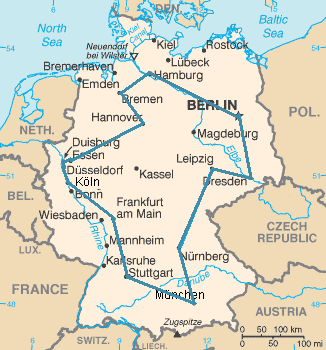
\includegraphics[width=0.8\textwidth]{TSP_Deutschland_3}
  \tiny

  user "Kapitän Nemo" \url{https://commons.wikimedia.org/w/index.php?curid=5584283}
\end{minipage}
\begin{minipage}{0.45\textwidth}

"Given a list of cities and the distances between each pair of cities, what is the shortest possible route that visits each city exactly once and returns to the origin city?"
\cite{song_solving_2021}
\end{minipage}
\end{frame}

\begin{frame}{Travelling Salesman Problem Definition}
  \begin{itemize}
    \item input graph
      \begin{itemize}
        \item weighted, non-negative
        \item undirected
        \item complete (fully connected)
      \end{itemize}

    \pause
    \item output restrictions:
      \begin{itemize}
        \item tour (cycle that visits every vertex)
        \item use any edge \emph{at most} one time
      \end{itemize}
    \pause
    \item problem: find a legal output that has minimal (cumulative) edge weight
  \end{itemize}
  \pause
  note: we do not assume the triangle inequality
\end{frame}

\begin{frame}{Why is TSP interesting?}
  \begin{itemize}
    \item well studied
    \item NP-complete $\rightarrow$ ressource intensive
    \item intuitive to understand
    \pause
    \item practical applications (see \href{https://en.wikipedia.org/wiki/Concorde_TSP_Solver}{Concorde TSP Solver})
  \end{itemize}
  % https://upload.wikimedia.org/wikipedia/commons/c/c4/TSP_Deutschland_3.png
\end{frame}


\section{Project Plan}

\begin{frame}[t]{Technical Decisions}
\begin{itemize}
\item \textbf{Programming Language:} Rust
\pause
\item \textbf{Input Format:} TSPLIB
\pause
\item \textbf{Project Scope:}
\begin{itemize}
\pause
\item I/O management
\pause
\item Exact solving
\begin{itemize}
\item Complete search
\item Search space pruning
\item Dynamic Programming
\end{itemize}
\pause
\item Approximation algorithms
\begin{itemize}
\item MST-based
\item Ant Colony Optimization
\end{itemize}
\pause
\item Lower bounds computation (MST based)
\pause
\item Post-Optimization (2-opt)
\end{itemize}
\end{itemize}
\end{frame}

\begin{frame}[t]{Timeline}
  \pause
\begin{itemize}
  \item Intial single threaded MVP:
  \begin{itemize}
    \item Input parser
    \item Naive exact solver
    \item Initial benchmarking using criterion
  \end{itemize}
  \pause
  \item Initial approximation approaches:
  \begin{itemize}
    \item MST-based approach
    \item Ant colony optimization
  \end{itemize}
  \pause
  \item Optimizing single threaded code
  \begin{itemize}
    \item Algorithmic improvements
    \item Classical Performance Engineering
  \end{itemize}
  \pause
  \item Inter-Node, Shared Memory Parallelization
  \begin{itemize}
    \item crossbeam, Rayon (OpenMP-alike)
  \end{itemize}
\end{itemize}
\end{frame}

\begin{frame}[t]{Timeline (cont.)}
\begin{itemize}
\item Optimizing Shared Memory Parallelization
  \begin{itemize}
    \item Evaluate Causal Profiling
  \end{itemize}
\pause
\item Intra-Node, Distributed Memory Parallelization
\begin{itemize}
\item rsmpi
\end{itemize}
\pause
\item Optimizing Distributed Memory Parallelization
\pause
\item Report Writing
\end{itemize}
\end{frame}


\begin{frame}{References}
    % References slide in appendix
    \renewcommand*{\bibfont}{\normalfont\scriptsize}
    \printbibliography[heading=none]
\end{frame}

\end{document}
